%%%%%%%%%%%%%%%%%%%%%%%%%%  phdsymp_sample2e.tex %%%%%%%%%%%%%%%%%%%%%%%%%%%%%%
%% changes for phdsymp.cls marked with !PN
%% except all occ. of phdsymp.sty changed phdsymp.cls
%%%%%%%%%%                                                       %%%%%%%%%%%%%
%%%%%%%%%%    More information: see the header of phdsymp.cls   %%%%%%%%%%%%%
%%%%%%%%%%                                                       %%%%%%%%%%%%%
%%%%%%%%%%%%%%%%%%%%%%%%%%%%%%%%%%%%%%%%%%%%%%%%%%%%%%%%%%%%%%%%%%%%%%%%%%%%%%%


%\documentclass[10pt]{phdsymp} %!PN
%\documentclass[twocolumn]{phdsymp} %!PN
%\documentclass[12pt,draft]{phdsymp} %!PN
%\documentstyle[twocolumn]{phdsymp}
%\documentstyle[12pt,twoside,draft]{phdsymp}
%\documentstyle[9pt,twocolumn,technote,twoside]{phdsymp}
\documentclass[a4paper,oneside,12pt]{article}

\usepackage{pdfpages}
\usepackage{a4wide}
\usepackage[english]{babel} 
\usepackage{url}
\usepackage{caption}
\usepackage{multirow}
\usepackage{rotating}
\usepackage{soul}
 
\usepackage{palatino}

\usepackage{graphicx}
\graphicspath{{figures/}} 
\def\BibTeX{{\rm B\kern-.05em{\sc i\kern-.025em b}\kern-.08em
    T\kern-.1667em\lower.7ex\hbox{E}\kern-.125emX}}

\newtheorem{theorem}{Theorem}

% zet de paragrafen een beetje uit elkaar en links uitgelijnd
\setlength{\parindent}{0mm}
\setlength{\parskip}{1ex plus 0.5ex minus 0.2ex} 

\setlength{\textheight}{23cm}
\setlength{\textwidth}{16cm}
\setlength{\oddsidemargin}{0cm}
\setlength{\evensidemargin}{0cm}
\setlength{\topmargin}{-1cm}

\penalty-10000
\tolerance=10000

% \setlength{\parskip}{0pt}
% \setlength{\parsep}{0pt}
% \setlength{\headsep}{0pt}
% \setlength{\topskip}{0pt}
% \setlength{\topmargin}{0pt}
% \setlength{\topsep}{0pt}
% \setlength{\partopsep}{0pt}

\linespread{0.9725}

\usepackage[compact]{titlesec}
%\titlespacing{\section}{1pt}{*0}{*0}
%\titlespacing{\subsection}{1pt}{*0}{*0}
\titlespacing{\subsubsection}{1pt}{*0}{*0}

\usepackage{mdwlist}

\begin{document}


%-------------------------------------------------------------------------------------------

\thispagestyle{empty}

\begin{center}
\mbox{}\\\vspace{5mm}
{\Large Application for China Scholarship Council Grant}\\ [45mm]
%
{\bf\Huge Hardware acceleration for\\
[3mm] FPGA CAD Tools} \\
\vspace{45mm}
\Large Yun Zhou \\
\vspace{2mm}
\small\texttt{email@address.com} \\
\vspace{20mm}
\Large Advisor: ir.\ Elias Vansteenkiste \\
\small\texttt{Elias.Vansteenkiste@ugent.be} \\
\vspace{2mm}
\Large Promotor: prof.\ dr.\ ir.\ Dirk Stroobandt \\
\small\texttt{Dirk.Stroobandt@ugent.be} \\
\vspace{20mm}
\normalsize Ghent University, Belgium \\
\normalsize Department of Electronics and Information Systems\\
\normalsize Computer Systems Lab\\
\normalsize Hardware and Embedded Systems Group 
\end{center}

%-------------------------------------------------------------------------------------------



%\title{Applying parameterizable dynamic configurations to sequence alignment} %!PN

%\author{Tom Davidson\thanks{T.~Davidson is with the Electronics and Information Systems department, Ghent University (UGent), Gent, Belgium. E-mail: tom.davidson@UGent.be .}, Karel Bruneel, Harald Devos, Dirk Stroobandt }

%%\title{Geautomatiseerde run-time-herconfiguratie van op het algoritmisch niveau}
%%\author{Elias Vansteenkiste}


%%\maketitle

\newpage

\tableofcontents

\clearpage

\section{Problem}
\hl{(1 page)}
A Field Programmable Gate Array (FPGA) is an integrated circuit made up of a grid of programmable functional blocks embedded in a programmable interconnection network. An FPGA can be programmed to implement any arbitrary logic function in the same way as Application Specific Integrated Circuits (ASICs), however the functionality of an FPGA is not fixed during the production process. The functionality can be changed by writing a different configuration to the configuration memory. This flexibility leads to a substantial reduction of the economic risk of developing hardware accelerators for FPGAs. It also explains the rise in the popularity of the FPGA \cite{}. \hl{we need a reference here} Unfortunately the flexibility of the FPGA comes at a price.  Each time the application developer wants to test his design. The design has to be compiled to a FPGA configuration and this is a complex process, that consist of multiple steps. In each step  multiple NP hard problems. 

Een FPGA is een ge\"integreerde schakeling (IC) die bestaat uit een rooster van programmeerbare logische blokken ingebed in een programmeerbaar interconnectienetwerk. Net als bij toepassingsspecifieke IC's (ASIC's) kan op een FPGA een arbitraire logische schakeling ge\"implementeerd worden. In ASIC's wordt de schakeling vast in de chip gebakken. De logische schakeling die een FPGA implementeert daarentegen, wordt bepaald door de inhoud van zijn configuratiegeheugen. Het grote voordeel van FPGA's is dat de logische schakeling eenvoudig kan veranderd worden door het configuratiegeheugen te herschrijven. Deze flexibiliteit zorgt voor een sterk verlaagd economisch risico (tegenover ASIC's) en daardoor groeit de populariteit van FPGA's. Jammergenoeg komt de programeerbaarheid van FPGA's met een prijs in de vorm van een grotere chipoppervlakte en een lagere kloksnelheid in vergelijking met ASIC's.

Summary: \emph{Dynamische FPGA-herconfiguratie biedt vele voordelen. Op dit moment kan enkel de functionaliteit, maar nog niet het interconnectienetwerk van de FPGA gespecialiseerd worden op een automatische manier. Dit leidt tot veel manueel werk op het architecturaal niveau en dus heel dure en niet-herbruikbare implementaties.} 

\newpage

\section{Goal}
\hl{What do you want to know, prove, demonstrate, analyse, test, investigate or examine? List your project aims in a logical sequence.}
\hl{(1 page)}

\emph{Het doel is het uitbreiden van de huidige automatische methode voor dynamische circuitspecialisatie met herconfiguratie van het routeringsnetwerk, zodat FPGA's nog effici\"enter gebruikt kunnen worden. Meer specifiek zal ik mij concentreren op het ontwikkelen van nieuwe plaastings- en routeringsmethoden die dit mogelijk maken.}

Conventioneel worden FPGA-configuraties gegenereerd in vier stappen: synthese, technologie-afbeelding (technology mapping), plaatsing en routering. De synthese neemt de hoogniveau-beschrijving van het digitaal systeem en vertaalt deze beschrijving naar een netlijst (een lijst van de logische poorten en de verbindingen ertussen). De technologie-afbeelding zet de netlijst om in een circuit met functionele blokken die aanwezig zijn op de doel-FPGA. De plaatsing wijst dan elk van de functionele blokken toe aan een fysieke functionele blok op de FPGA. Daarna routeert de routeerder de nodige connecties tussen de logische blokken. 

Om dynamische routering van interconnecties mogelijk te maken, moeten ook de voorafgaande stappen in de configuratiegeneratie aangepast worden. Tijdens de technologie-afbeelding worden TCON's of \mbox{{\em tunable connections}} ingevoerd. Een TCON is een verbinding tussen een bronpin en een doelpin, de verbinding moet actief zijn als voldaan is aan de connectievoorwaarde. De connectievoorwaarde is een boolese functie van de parameters. TCON's worden volledig door het programeerbaar interconnectienetwerk ge\"implementeerd. Opdat de routeerder dit effici\"ent zou kunnen doen, moet de plaatser eerst de logische blokken zo proberen te plaatsen dat de kost van de tussenliggende TCON's geminimaliseerd wordt, net als de kost van de gewone verbindingen tussen logische blokken. Hiervoor moet de plaatser de kost van een TCON kunnen voorspellen, uitsluitend gebruik makend van de posities van de functionele blokken.

Het prototype van een herconfiguratie-bewuste routeerden in mijn thesis~\cite{mthesiselias} heb ik uitgewerkt in de eerste termijn van mijn doctoraat. Deze routeerder kan een lijst van TCON's routeren. Sommige TCON's moeten nooit gelijktijdig gerealiseerd worden en mogen dus routeringsmiddelen delen. De routeerder gebruikt deze eigenschap om een compacte routering van de TCON te realiseren. Tijdens mijn eerste termijn heb ik in eerste instantie meer overlapmogelijkheden in het prototype van de routeerder mogelijk gemaakt zodat nog compactere routeringen te produceren. Eens de routeerder op punt stond heb ik het voorspellingsalgoritme van de plaatser afgestemd op het gedrag van de routeerder. De nieuwe technologie-afbeelder behoort niet tot mijn doctoraaatswerk, maar is ontwikkeld door andere onderzoekers aan onze onderzoeksgroep. De plaatser en routeerder worden op dit moment ingebouwd in academische tool flows om het mogelijk te maken onze techiek te testen op diverse FPGA-architecturen, waaronder de architecturen die op dit moment gebruikt worden in commerciële FPGA's

In de totale methodologie kunnen op dit moment enkel TCON's tussen logische blokken behandeld worden, geen ketens van TCON's. TCON's die rechtstreeks verbonden zijn met andere TCON's komen wel voor in vele toepassingen maar moeten dan eerst samengenomen worden tot een grotere TCON om de routering mogelijk te maken. Indien vele TCON's verbonden zijn, kan dit leiden tot extreem lange uitvoeringstijden. Dit probleem wil ik ook in de tweede termijn van mijn doctoraat aanpakken.

\newpage

\section{Background}
\hl{(4 pages)}
What is already known or unknown? Set the scene.

\subsection{Situering}

FPGA's worden steeds vaker gebruikt als componenten in digitale systemen. Zoals in de probleemstelling is vermeld, is de populariteit van FPGA's te danken aan de flexibiliteit die de (her)configureerbaarheid met zich meebrengt. Op een FPGA kan een willekeurige digitale schakeling ge\"implementeerd worden. De enige beperking is de grootte van de FPGA. Om dit mogelijk te maken bevat de FPGA een rooster van logische blokken. Elk logisch blok bevat op zijn beurt enkele Look-Up Tables (LUT's). Elke LUT kan om het even welke Boolese functie van zijn ingangen kan implementeren. Dit is mogelijk door de waarheidstabel van deze functie in het geheugen van de LUT te schrijven. De logische blokken zijn ingebed in een interconnectienetwerk dat volledig configureerbaar is. Dit interconnectienetwerk kunnen we configureren door bepaalde waarden te schrijven in de geheugencellen van de schakelaars. De geheugens van zowel de LUT's als de interconnecties vormen samen het configuratiegeheugen van de FPGA. 

\subsubsection{Conventional FPGA CAD tools}
In klassiek FPGA-ontwerp wordt de FPGA alleen geconfigureerd bij het opstarten of bij updates. Het configuratiegeheugen wordt dan geschreven aan de hand van een configuratiebitstroom. Het genereren van deze bitstroom is een complexe taak. Daarvoor werden geautomatiseerde toolflows ontwikkeld. Deze toolfows zetten een beschrijving van het systeem op RT-niveau om naar een configuratiebitstroom voor de FPGA. Dit gebeurt aan de hand van de volgende stappen (een overzicht is weergegeven in het schema links in Figuur \ref{toolflows}).

\paragraph{Synthesis}
De ontwerper beschrijft zijn digitaal systeem aan de hand van een hardwarebeschrijvingstaal (Hardware Description Language). De synthesestap vertaalt de beschrijving naar een netlijst van logische poorten, in- en uitgangen en netten.

\paragraph{Technology Mapping} 
De technologie-afbeelder beeldt de netlijst met poorten en netten af op een circuit met functionele blokken die aanwezig zijn op de doel-FPGA en netten die deze functionele blokken verbinden.

\paragraph{Placement}
De plaatser kiest een logisch blok op de FPGA voor elk functioneel blok in het circuit. De plaatser plaatst de blokken rekening houdend met een optimalisatiecriterium. Mogelijke optimalisatiecriteria zijn minimale draadlengte, routeerbaarheid en minimale vertraging. Deze optimalisatiecriteria zijn niet onafhankelijk van elkaar. In dit project wordt een draadlengte-gedreven plaatser beschouwd. Draadlengte-gedreven plaatsers proberen de blokken zo te plaatsen dat de routeerder een minimum aan routeringsmiddelen nodig heeft om de netten tussen de blokken te routeren.

Tijdens de plaatsing moet het plaatsingsalgoritme de kwaliteit van een plaatsing op elk moment kunnen inschatten. Als we optimaliseren voor minimale draadlengte, komt dit erop neer dat de plaatser moet voorspellen hoeveel routeringsmiddelen de routeerder zal nodig hebben. Hiervoor beschikt hij enkel over de posities van de functionele blokken. Om de routeringsmiddelen te schatten, zijn al vele kostenfuncties voorgesteld~\cite{vprBVRJ, vprboek}. Hoe beter de geschatte routeringsmiddelen overeenkomen met de eigenlijke routeringsmiddelen hoe beter de plaatser zijn werk kan doen.

\paragraph{Routing} Na de plaatsingsstap is de plaats van de logische blokken bekend en is er dus voldoende informatie beschikbaar voor het routeren van de netten in de op de FPGA aanwezige interconnectienetwerk. Het routeren van \'e\'en net is te herleiden tot het Steiner-boomprobleem (een bekend NP-compleet probleem dat door de routeerder opgelost wordt met een heuristiek).

Netten mogen geen routeringsmiddelen delen want dat zou een kortsluiting veroorzaken. De routeerder moet dus op zoek gaan naar disjuncte verzamelingen van routeringsmiddelen, voor elk net \'e\'en verzameling. De meeste conventionele routeerders voor FPGA~\cite{vprBVRJ, vprboek} doen dit aan de hand van het pathfinder-algoritme~\cite{pathfinder}. Dit is een iteratief algoritme waarbij de gerouteerde netten verschillende keren opgebroken en opnieuw gerouteerd worden. In de eerste iteratie houdt pathfinder weinig tot geen rekening met het overgebruik van routeringsmiddelen op bepaalde plaatsen (congestie). In de daaropvolgende iteraties verhoogt pathfinder geleidelijk de kost van routeringsmiddelen die overgebruikt worden tot er geen congestie meer is.

\begin{figure}[ht]
\centering
\includegraphics[width = 0.9\textwidth,trim = 0mm 10mm 0mm 55mm, clip]{toolflows.pdf}
\caption{Schematische voorstelling van de conventionele en de aangepaste toolflow. Dit doctoraat focust op de donkergrijs gekleurde stappen (TPlace en TRoute).}
\label{toolflows}
\end{figure}

\subsubsection{Run-time-herconfiguratie}\label{rtr}
Een FPGA (her)configureren is niet meer of minder dan de waarden van de configuratiebits in het configuratiegeheugen (her)schrijven. Zoals in de probleemstelling werd vermeld, wordt de herconfigureerbaarheid van de FPGA bij klassieke methodes zelden ten volle gebruikt. %, enkel bij het opstarten van de FPGA en bij updates.
De meeste SRAM-gebaseerde FPGA's kunnen echter geherconfigureerd worden tijdens de werking van de FPGA. Dit wordt {\em run-time-herconfiguratie} (RTR) genoemd. Sommige moderne FPGA's \cite{XilinxRTRFlow1,XilinxRTRFlow2} beschikken ook over parti\"ele herconfiguratiemogelijkheden. Bij parti\"ele RTR worden specifieke gebieden geherconfigureerd, terwijl de rest van de FPGA ongewijzigd blijft doorwerken. 

Om RTR mogelijk te maken moet het systeem naast een FPGA ook een configuratiemanager (CM) bevatten. De CM is verantwoordelijk voor het berekenen of selecteren van nieuwe configuraties en het herconfigureren van de FPGA. De belangrijkste reden om aan RTR te doen, is dat RTR in vele gevallen ervoor zorgt dat we de applicatie op een kleinere en dus goedkopere FPGA kunnen implementeren. De nodige hardware is immers kleiner dan in het klassieke geval waarbij voor elke functionaliteit een apart hardwareblok moet gereserveerd worden. We kunnen ook een even grote FPGA blijven gebruiken. In dat geval hebben we meer parallellisme ter beschikking voor het verbeteren van de uitvoeringstijd.

\paragraph{Geparameteriseerde configuratie}
De techniek van geparameteriseerde configuraties is een ontwerpsmethode voor parti\"ele RTR. Deze techniek werd ontwikkeld binnen de onderzoeksgroep CSL/HES aan de UGent, met als doel het mogelijk maken van herconfiguratie met fijne granulariteit. Een bijkomend doel  is de techniek gemakkelijk toegankelijk maken voor de ontwerper door de ontwerpsbeslissingen omtrent RTR op een hoog abstractieniveau te houden. Conceptueel komt de techniek neer op het indelen van de ingangssignalen in 2 groepen: de parameters en de overige ingangssignalen. De ontwerper kiest de traag vari\"erende signalen als parameters door ze te annoteren in de hardwarebeschrijving. De aangepaste toolflow, te zien in Figuur~\ref{toolflows} (rechts), genereert dan automatisch een geparameteriseerde bitstroom (PBS) op basis van de hardwarebeschrijving op RT-niveau. De PBS is een bitstroom waarin sommige bits uitgedrukt zijn als Boolese functies van de parameters. Telkens een parameterwaarde verandert, zal de CM de PBS herevalueren om zo een gespecialiseerde configuratiebitstroom te verkrijgen die dan gebruikt wordt om de FPGA te herconfigureren. De uiteindelijke FPGA-implementatie wordt op die manier kleiner en sneller.

\paragraph{Het genereren van een geparameteriseerde configuratie}

Op dit moment bestaat er een geautomatiseerde methode die toelaat een geparameteriseerde configuratie te genereren die de waarheidstabellen van de LUTs uitdrukt in functie van de parameters. Deze LUT's worden Tunable LUT's (TLUT's) genoemd. Bij deze methode blijven de routeringsconfiguratiebits constant. In mijn doctoraat wil ik ook de routeringsbits uitdrukken in functie van de parameters. De gebruikte oppervlake kan hierdoor verder gereduceerd worden.

\subsection{Mijn onderzoek}

De interconnectiestructuur van een FPGA bestaat uit draden en schakelaars. Een connectie tussen twee logische blokken wordt gemaakt door een aantal schakelaars te sluiten. Dit is mogelijk door de juiste bitwaarden te schrijven in de geheugencellen die deze schakelaars controleren. Door deze bitwaarden uit te drukken als functie van de parameters, bepalen de parameters wanneer een connectie geactiveerd wordt en wanneer niet. Deze parameterafhankelijke connectie noemen we een {\em Tunable Connection} (TCON). 

\paragraph{De TCON als basis}
Een TCON wordt gedreven door 1 bron en heeft 1 doel. Op het niveau van een tunable circuit kan de TCON gezien worden als een abstracte verzameling van routeringsmiddelen die de connectie realiseren als de connectievoorwaarde voldaan is. De parameters van een TCON bepalen dan welke connectie op welk moment geactiveerd wordt. Als een connectie geactiveerd wordt, moeten alle schakelaars die deze connectie realiseren, sluiten. Een voorbeeld van een functionaliteit die kan voorgesteld worden door TCON's is schematisch voorgesteld in de Figuur~\ref{tconschema}. Dit voorbeeld heeft twee ingangen $i_0$ en $i_1$, en twee uitgangen $o_0$ en $o_1$. Voor elke waarde van de parameter $p_0$ is te zien welke connecties geactiveerd moeten worden.

\begin{figure}[ht]
\centering
\includegraphics[width = 0.9\textwidth,trim = 0mm 0mm 0mm 115mm, clip]{tconschema.pdf}
\caption{Een schematische voorstelling van een 2-wegsschakelaar en de connecties voor de verschillende waarden van de parameters actief moeten zijn.}
\label{tconschema}
\end{figure}

In de situering werden de voordelen van het gebruik van TCON's al aangehaald. Ik zet ze hier nog eventjes op een rij.
\begin{itemize}
\item \textbf{Het reduceren van de benodigde FPGA-oppervlakte}: TCON's leiden tot geparameteriseerde configuraties waarbij de routeringsbits dynamisch geherconfigureerd worden. Deze configuraties zijn compacter omdat het aantal benodigde LUT's daalt tegenover configuraties zonder TCON's. 
\item \textbf{Het reduceren van de benodigde routeringsmiddelen}: De routeringsmiddelen van de FPGA zijn heel schaars en meestal een beperkende factor bij het plaatsen van een circuit op een FPGA. De routeringsinfrastructuur schaalt ook slecht, daardoor treden problemen op bij de nieuwste FPGA's waarbij het aantal blokken toeneemt. Bij het routeren van TCON's kan de routeerder het aantal benodigde routeringsmiddelen minimaliseren. Dit is mogelijk door het delen van routeringsmiddelen tussen connecties die mogen overlappen te stimuleren. Connecties die niet gelijktijdig actief zijn en connecties die dezelfde ingang hebben mogen routeringsmiddelen delen.
\item \textbf{Lagere configuratietijden}: Het delen van routeringsmiddelen heeft als gevolg dat er minder te herconfigureren routeringsbits zijn, omdat deze samenvallen.
\item \textbf{De logische diepte van het circuit daalt}, waardoor het systeem sneller wordt.
\end{itemize}

\renewcommand{\arraystretch}{1.2} 
\renewcommand{\tabcolsep}{0.20cm} 
\begin{table}[t]
\caption{Eigenschappen van de verschillende Clos-netwerk implementaties}
\label{tbl:clos}
\centering
\begin{tabular}{rlrrrrrrr}
\textbf{Grootte}&\textbf{Type Impl}&\begin{sideways}Oppervlakte(LUTs)\end{sideways}&\begin{sideways}FPGA Dimensie\end{sideways}&\begin{sideways}Logische Diepte\end{sideways}&\begin{sideways}Min. kanaalbreedte\end{sideways}&\begin{sideways}Totale draadlengte\end{sideways}&\begin{sideways}Run-time Plaatser\end{sideways}&\begin{sideways}Run-time Routeerder\end{sideways}\\
%\textbf{Grootte}&\textbf{Type implementatie}&\textbf{Oppervlakte}&\textbf{Dimensie FPGA}&\textbf{Logische Diepte}&$\textbf{Min. kanaalbreedte}$&\textbf{Totale Draadlengte}&$\textbf{Compilatietijd}_{plaatser}$&$\textbf{Compilatietijd}_{routeerder}$\\
\hline
\hline
\multirow{3}{*}{16} 	&Conventioneel	&202	&$20\times 20$	&5	&6	&2340		&5.3s	&6.3s\\
					&TLUT	&48		&$10\times 10$		&3	&6	&492		&0.6s	&0.5s\\
					&TCON	&16		&$8\times 8$		&1	&6	&453		&1.5s	&1.1s\\
\hline
\multirow{3}{*}{64} 	&Conventioneel	&1016	&$47\times 47$	&9	&8	&11941		&1m15s		&6m43s\\
					&TLUT	&320	&$23\times 23$	&5	&9	&3129		&11s		&28s\\
					&TCON	&128	&$18\times 18$	&2	&16	&4289		&20s		&1m12s\\
\hline
\multirow{3}{*}{256} 	&Conventioneel	&6760	&$114\times 114$	&12	&10	&98471		&39m27s	&7h1m2s\\
					&TLUT	&1792 	&$53\times 53$		&7	&14	&23612		&2m50s		&28m15s\\
					&TCON	&768 	&$39\times 39$		&3	&28	&30579		&5m33s		&1h39m11s\\
\hline
\end{tabular}
\end{table}

Als voorbeeld bekijken we de implementatie van een clos-netwerk. Clos-netwerken zijn netwerken die alle ingangen met alle uitgangen verbinden via een schakelnetwerk. Dit schakelnetwerk is een voorbeeldapplicatie waarmee we de verschillende methodes kunnen vergelijken. Voor de implementatie van clos-netwerken heeft de geparameteriseerde configuratie met TLUT's 4 keer minder oppervlakte nodig dan de conventionele implementatie zonder RTR, omdat het aantal benodigde LUT's daalt~\cite{phdkarel}. Een geparameteriseerde configuratie met TCON's en TLUT's kan de benodigde oppervlakte verder reduceren met een factor 8 tot 13. In Tabel~\ref{tbl:clos} zijn de resultaten te zien voor de TCON, de TLUT en de conventionele implementatie. Een kanttekening die gemaakt moet worden bij deze applicatie is dat de compilatietijd omhoog gaat en ook de kanaalbreedte. De meerkost in kanaalbreedte kan wel sterk verminderd worden door een klein deel van de oppervlaktewinste in te geven en de routering meer te spreiden zodat lagere kanaalbreedtes bereikt kunnen worden. Een ander nadeel is de hogere compilatietijd voor het genereren van een geparamteriseerde configuratie, maar als het per gespecialiseerde configuratie bekijken dan valt dit goed mee. 

%{
\renewcommand{\arraystretch}{1.2} 
\renewcommand{\tabcolsep}{0.17cm} 
\begin{table}[t]
\caption{Eigenschappen van Reguliere Expressie herkenner voor drie verschillende grid groottes} %\hl{(TLUT implementation?)}}
\label{tbl:expressionmatcher}
%\begin{center}
\begin{tabular}{clrrrrrrr}
\textbf{Grootte}&\textbf{Type Impl}&\begin{sideways}Oppervlakte(LUTs)\end{sideways}&\begin{sideways}FPGA Dimensie\end{sideways}&\begin{sideways}Logische Diepte\end{sideways}&\begin{sideways}Min. kanaalbreedte\end{sideways}&\begin{sideways}Totale draadlengte\end{sideways}&\begin{sideways}Run-time Plaatser\end{sideways}&\begin{sideways}Run-time Routeerder\end{sideways}\\
%\textbf{Size}&\textbf{Impl}&\textbf{Area}&\textbf{Dim}&$\textbf{CW}_{min}$&\textbf{WL}&$\textbf{RT}_{place}$&$\textbf{RT}_{route}$\\
\hline
\hline
\multirow{2}{*}{$4\times4$} 	&Conventioneel	&1141		&$38\times38$		&8 	&6		&5989		&53s		&43s\\
							&TCON			&577 		&$27\times27$		&3	&6		&4139		&29s		&19s\\
\hline
\multirow{2}{*}{$8\times8$} 	&Conventioneel	&4581		&$75\times75$		&8	&6		&26428		&11m46s	&10m44s\\
							&TCON			&2305 		&$53\times53$		&3	&7		&17768		&6m42s		&7m50s\\
\hline
\multirow{2}{*}{$14\times14$} 	&Conventioneel	&14061		&$130\times130$	&8	&6		&86328		&1h18m11s	&2h44m45s\\
							&TCON			&7057 		&$93\times93$		&3	&8		&55049		&1h0m45s	&1h24m2s\\
\hline
\end{tabular}
%\end{center}
\end{table}
%}


Een andere voorbeeld applicatie die ik getest heb in mijn eerste termijn is een virtuele grofmazige herconfigureerbare architectuur voor het herkennen van een reguliere expressie. Dit is vooral belangrijk in netwerk intrusie detectie systemen met pakket inspectie. In tabel, is te zien dat de TCON implementatie superieur is in zowel oppervlakte (benodigde LUTs), logische diepte als compilatietijd. 

Het probleem dat ik in mijn eerste termijn van mijn doctoraat opgelost heb  is een geparameteriseerde configuratie met geparameteriseerde connecties (TCONs) op een automatische manier te genereren. Op deze manier is het mogelijk om geparameteriseerde configuraties te genereren waarbij ook de routeringsbits uitgedrukt worden in functie van de parameters.
Ik heb de oplossing beschreven en voorgesteld in publicaties op belangrijke FPGA-gerelateerde conferenties zoals, het 8ste Internationaal Symposium over `Applied Reconfigurable Computing' (ARC2012)~\cite{connectionrouter} en de 22ste internationale conferentie over `Field Programmable Logic and Applications' (FPL2012)~\cite{vansteenkiste2012}.

\paragraph{Aanpassingen aan de toolflow}

Net zoals bij de geparameteriseerde configuratietoolflow voor TLUT's, moet de ontwerper in de hardwarebeschrijving voor de gecombineerde TCON-TLUT toolfow aanduiden welke signalen parameters zijn. De synthesestap vertaalt deze geannoteerde hardwarebeschrijving naar een netlijst. %die nu naast poorten, netten, de normale in- en uitgangen ook parameters bevat. 
De technologie-afbeelder beeldt dit poortnetwerk nu af op een aanpasbaar circuit, een {\em tunable circuit}, dat bestaat uit een TLUT's en andere gespecialiseerde hardware blokken ge\"interconnecteerd door TCON's. De technologie-afbeelder is geen onderdeel van mijn doctoraat. Een methode voor een nieuwe technologie-afbeelder is voorgesteld is uitgewerkt in \cite{tconmap} door een andere doctoraatsstudent in onze onderzoeksgroep CSL/HES.

Na de synthese werken de plaatser en de routeerder de vooralsnog abstracte TCON's verder uit. De plaatser plaatst de LUT's en TLUT's op de FPGA. Na de plaatsing is de plaats van de in- en uitgang van iedere TCON gekend. De routeerder routeert dan de TCON's. Na de routering zijn ook alle draden en schakelaars gekend die de TCON's realiseren. Sommige schakelaars en draden kunnen gedeeld worden door TCON's die niet gelijktijdig actief zijn of door connecties die dezelfde ingang hebben. De routeerder zal deze eigenschap gebruiken voor het minimaliseren van de benodigde routeringsmiddelen. %Dit is een zeer interessante uitdaging omdat de routeringsmiddelen op een FPGA zeer schaars zijn. 

In de eerste termijn van mijn doctoraat heb ik me toegespitst op het uitwerken van TCON's, waarbij het delen van routeringsmiddelen gemaximaliseerd wordt. Het uitwerken van deze methode bevatte twee stappen, het ontwikkelen van een nieuwe herconfiguratie-bewuste routeerder en het ontwikkelen van een nieuwe herconfiguratie-bewuste plaatser.


\subsubsection{Herconfiguratie-bewuste routeerder}\label{router}

Aangezien de routeringsschattingen in de plaatser afhankelijk zijn van de routeerder, was de eerste stap in mijn onderzoek het ontwikkelen van een herconfiguratie-bewuste routeerder die in staat is TCON's te routeren. Ik wijzigde het bestaande pathfinder-algoritme zodat deze TCON's routeert afzonderlijk. Om plaatswinst te boeken, worden connectiesegmenten zoveel mogelijk hergebruikt door schakelaars te delen tussen connecties die niet tegelijkertijd actief zijn (en dus afhankelijk zijn van verschillende parameterwaarden). Een gedeelde schakelaar moet dus gesloten worden voor meerdere parameterwaarden. Elke schakelaar zal zijn eigen sluitingsvoorwaarde hebben. 
Het delen van routeringsmiddelen kan tot compactere implementaties leiden, zoals te zien is in de voorgaande tabellen met resultaten. In Figuur~\ref{tcon} is te zien hoe het voorbeeld, de 2-wegsschakelaar uit Figuur~\ref{tconschema} ge\"implementeerd kan worden op een FPGA met 2x2 logische blokken. Bij iedere schakelaar is de sluitingsvoorwaarde afgebeeld. De gedeelde schakelaars hebben een sluitingsvoorwaarde 1 en moeten niet geherconfigureerd worden. Dit leidt tot lagere herconfiguratietijden.

\begin{figure}%[ht]
\centering
\includegraphics[width = 0.65\textwidth,trim = 0mm 0mm 0mm 35mm, clip]{tcon.pdf}
\caption{Een schematische voorstelling van een TCON en de implementatie van deze TCON op een FPGA  met 2x2 logische blokken. De draden van de routeringsstructuur zijn voorgesteld door dikke lijnen, de schakelaars door dunne lijnen. De schakelaars en draden gebruikt voor het realiseren van de TCON worden zwart gekleurd. Bij iedere gebruikte schakelaar is de sluitingsvoorwaarde afgebeeld.}
\label{tcon}
\end{figure}

%Dit prototype gaat ervan uit dat de connecties in een TCON die niet gelijktijdig actief zijn en connecties die dezelfde bron hebben, routeringsmiddelen mogen delen. Voor het uitbuiten van deze eigenschap gebruikt het prototype een paar vereenvoudigde regels. De eerste regel is dat connecties mogen overlappen als ze dezelfde bron hebben. De tweede regel is dat connecties mogen overlappen als ze hetzelfde doel hebben. Deze laatste regel is geldig omdat connecties met hetzelfde doel nooit gelijktijdig kunnen voorkomen, anders zou kortsluiting mogelijk zijn. Dit eerste prototype is beperkt en wil ik uitbreiden. Een eerste uitbreiding heeft als bedoeling om nog effici\"entere implementaties te genereren. In de tweede uitbreiding zal ik de ondersteuning voor de verschillende FPGA architecturen uitbreiden. 


%Het prototype gebruikt een paar vereenvoudigde regels om de routeringsmiddelen te delen maar is hierin zeer beperkt. 
%Een eerste beperking van het prototype is dat niet alle overlapmogelijkheden ontdekt worden, zoals te zien is in Figuur~\ref{overlapmogelijkheden}. Op deze figuur is een TCON afgebeeld met twee connecties. Aangezien deze connecties geen gemeenschappelijk doel of bron hebben, worden ze volledig gescheiden gehouden. Toch mogen deze twee connecties routeringsmiddelen delen, want ze moeten niet geactiveerd worden op hetzelfde moment. Tijdens mijn doctoraat zal ik het prototype uitbreiden zodat de routeerder dergelijke overlapmogelijkheden uitbuit. Ik zal ook onderzoeken op welke manier de routeerder het delen van routeringsmiddelen het best stimuleert. Bij dit deel zal het belangrijk zijn de complexiteit van het routeringsalgoritme in het oog te houden. 


%Een eerste uitbreiding heeft als bedoeling om nog effici\"entere implementaties te genereren. In de tweede uitbreiding zal ik de ondersteuning voor de verschillende FPGA architecturen uitbreiden. 

% Misschien gaat deze sectie te technisch. We zullen zien. Als we te weinig plaats hebben kan dit eruit.
%\paragraph{Optimalisaties} We kunnen de connectierouteerder nog verder optimaliseren. Bepaalde optimalisaties zijn mogelijk omdat pathfinder voor iedere connectie slechts \'e\'en doel moet vinden. Een eerste optimalisatie is het gebruik van twee verkenningsgolven in plaats van \'e\'en, \'e\'en met als oorsprong de bron van de connectie en \'e\'en met als oorsprong het doel van de connectie. Op deze manier zullen minder routeringsmiddelen verkend worden totdat het kortste pad gevonden is. Een tweede mogelijke optimalisatie is de BFS-verkenningsstrategie (Breadth First Search) vervangen door het A*-algoritme. Deze optimalisatie zorgt ervoor dat de verkenningsgolf vervormt wordt zodat het kortste pad sneller gevonden wordt.

\subsubsection{Herconfiguratie-bewuste plaatser}\label{plaatser}

De conventionele plaatser is niet in staat om functionele blokken die verbonden worden door TCON's goed te plaatsen op een FPGA. In de eerste fase van mijn doctoraat ben ik al begonnen met het ontwikkelen van een herconfiguratie-bewuste draadlengte-gedreven plaatser. Ik heb onderzocht op welke manier de plaatser de functionele blokken moeten plaatsen zodat het aantal benodigde routeringsmiddelen voor het realiseren van de TCON's geminimaliseerd wordt.

De conventionele plaatsers voorspellen de benodigde routeringsmiddelen van een plaatsing door in te schatten hoeveel routeringsmiddelen de verschillende netten afzonderlijk nodig zullen hebben, aan de hand van de bounding box van dat net. Een bounding box (BB) van een net is de minimale rechthoek die alle eindpunten van een net bevat. Het schatten op basis van individuele netten is mogelijk omdat netten niet mogen overlappen en de routering van een circuit eigenlijk de samenstelling is van de verschillende gerouteerde netten. Als overlap mogelijk wordt, zal de conventionele plaatser de kost van een net dus te hoog inschatten en bijgevolg niet de beste positie voor de verbonden logische blokken kiezen. 

\begin{figure}
\centering
\includegraphics[width = 0.7\textwidth,trim = 0mm 30mm 0mm 25mm, clip]{BBconnectieFPGAplusimplementatie.pdf}
\caption{%Schematische voorstelling van een FPGA met 4x4 logische blokken.\\(a) 
De bounding box van een connectie kan op verschillende manieren gedefinieerd worden, al dan niet rekening houdend met de verschillende overlapmogelijkheden (a). In (b) staat een implementatie van de connecties in (a) die kan gegenereerd worden door de connectierouteerder}
\label{BBconnectieFPGAplusimplementatie}
\end{figure}

In de nieuwe herconfiguratie bewuste plaaster, worden de connecties onderverdeeld in groepen volgens het belangrijkste routeringsmiddelen delingsmechanisme. Connecties die overwegend draadjes delen met connecties die dezelfde bron hebben worden zoveel mogelijk samengenomen. Omgekeerd geldt hetzelfde. Na de onderverdeling is een elke connectie lid van \'e\'en groep.
Het aantal benodigde routeringsmiddelen van een tunable circuit wordt dan voorspelt door in te schatten hoeveel routeringsmiddelen nodig zijn voor elke groep. Hierbij passen we de BB-definities toe die bij conventionele plaatsers gebruikt worden. Dit voorspellingsalgoritme voor de routeringskost haalt hoge correlaties met de effectieve routeringskost.

De plaaster is samen met routeerder beschreven in een journal manuscript die op dit moment in overweging wordt genomen als kandidaat publicatie voor het IEEE 'Transactions on Computer-Aided Design' tijdschrift. 

%\paragraph{Optimalisaties} Na het ontwikkelen van een herconfiguratie-bewuste draadlengte-gedreven plaatser kan deze uitgebreid worden met andere optimalisatiecriteria, zoals routeerbaarheid en minimale vertraging.
\newpage
\section{Feasibility}
Expected outcomes, significance or rationale
Why is it important? 
What do you expect it will deliver? 
What are the expected outcomes? 
Establish the importance of your project by highlighting its originality or why it is worth pursuing. Highlight the benefits, positive expected outcomes or innovative applications of knowledge.


\subsection{Context and Strategy}\label{context}
My research will be conducted at Ghent University in the research group Hardware and Embedded Systems (HES). HES is part of the Computer Systems Lab (CSL) in the Department of Electronics and Information Systems. The HES group is lead by professor Dirk Stroobandt. The group has a lot of experience with developping FPGA CAD tool software.

\newpage

\section{Timetable}\label{timetable}
\hl{(1 page)}
Indicate the timeframe for each broad stage considering literature surveys, data collection, production, modelling, review, analysis,
testing, reporting, chapter and thesis writing, and thesis submission date.

The research in this project will be divided in 2 big stages:

\subsection{Work Packages}
\begin{description*}
\item[Hardware Acceleration of the placement phase(18 maanden)]\

\begin{description*}
\item[De connectie-gebaseerde routeerder (8+1 maanden)]\
In het eerste onderdeel zal het prototype verder ontwikkeld worden via de uitbreidingen die eerder beschreven zijn. Na dit deel zal een maand tijd uitgetrokken worden voor het rapporteren over de connectie-gebaseerde routeerder
\item[De connectie-gebaseerde plaatser (8+1 maanden)]\
Na het ontwikkelen van de routeerder kunnen we de plaatser erop afstemmen. Er is ook 1 maand gereserveerd voor het rapporteren over de nieuwe plaatsingsalgoritmes.
\end{description*}

\item[Hardware Acceleration of the the routing phase (17 maanden)]\

\begin{description*}
\item[Aanpassingen aan de herconfiguratie-bewuste routeerder (8 maanden)] 
We beginnen met een nieuw routeringsalgoritme dat op een schaalbare manier kan omgaan met een aaneenschakeling van TCON's.
\item[Aanpassingen aan de herconfiguratie-bewuste plaatser (8+1 maanden)]
De plaatser zal in deze fase opnieuw aangepast worden aan de eerder ontwikkelde routeerder. Na deze stap volgt een maand voor het rapporteren over de aaneenschakeling van TCON's.
\end{description*}

\item[Writing the doctoral thesis and reporting final results. (6 months)] This time is allocated to write the thesis and to report the finalized results in journals and conferences.  

\end{description*}

\begin{figure}[ht]
\centering
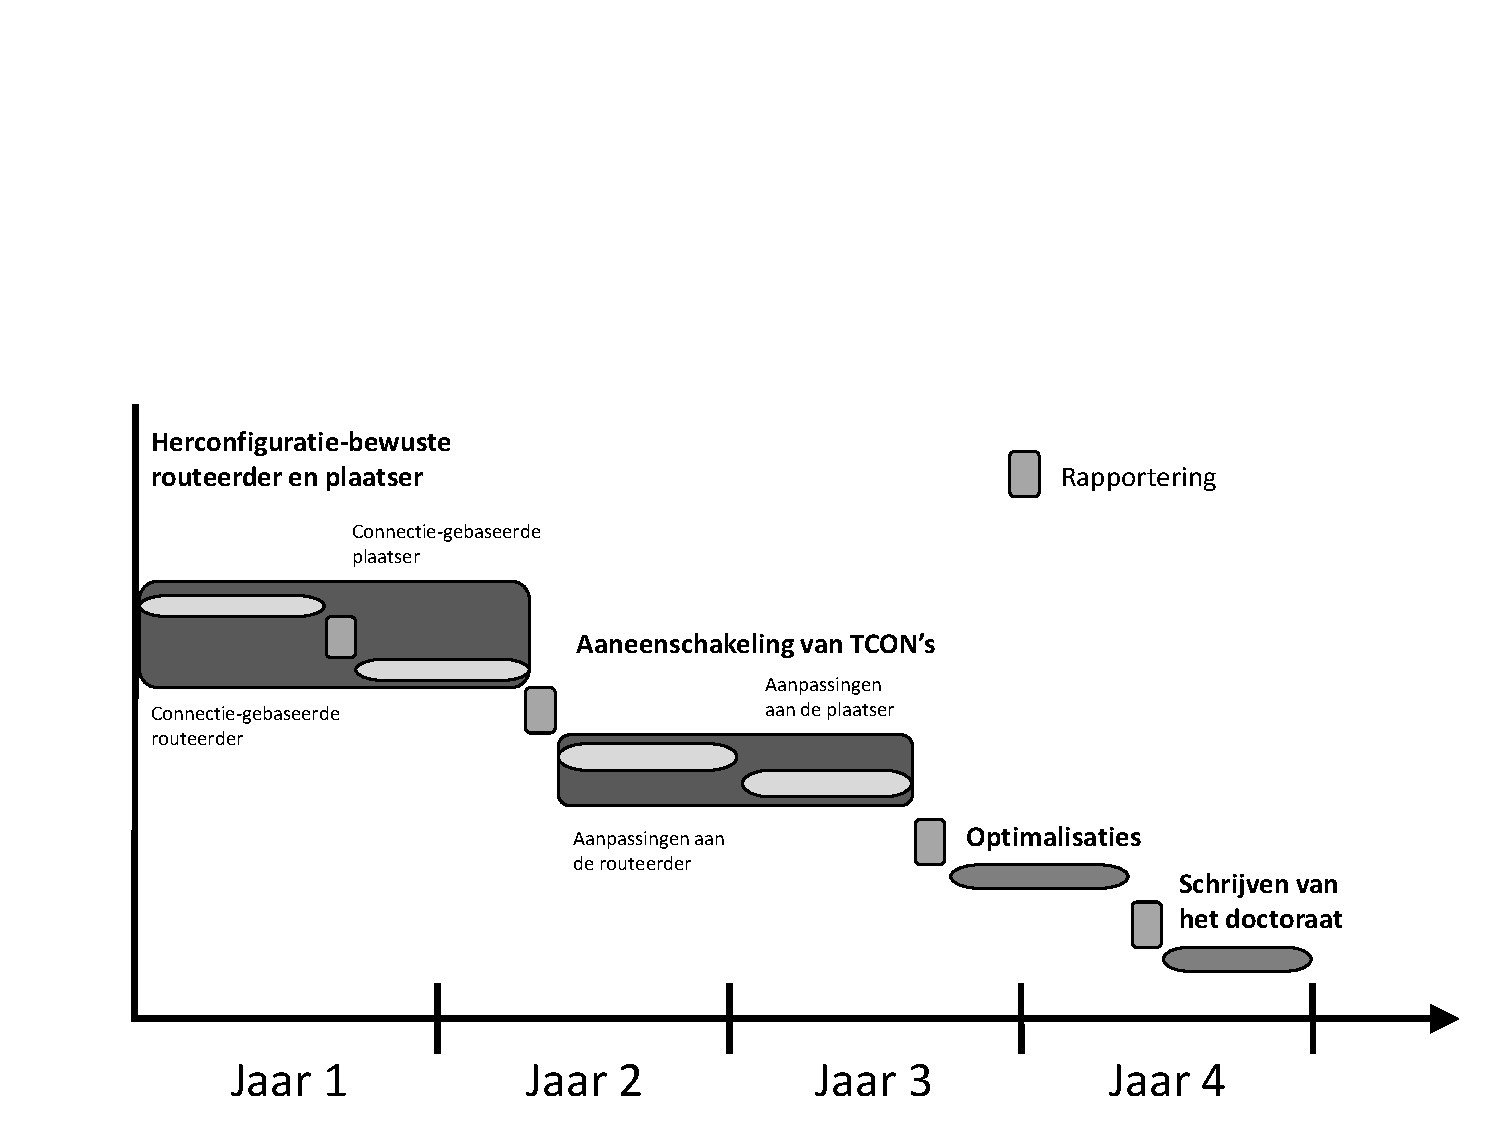
\includegraphics[width = \textwidth,trim = 0mm 0mm 0mm 70mm, clip]{tijdschema.pdf}
\end{figure}

\newpage


%\nocite{*}
\bibliographystyle{phdsymp}
\bibliography{AanvraagIWT} % commented if *.bbl file included, as
%\bibliography{../../../bib/hes} % commented if *.bbl file included, as
%%%%%see below
%%DIrk_bis: in je referenties hoofdletters escapen door ze tussen {} te zetten, zoals voor {FPGA}'s.

%%%%%%%%%%%%%%%%% BIBLIOGRAPHY IN THE LaTeX file !!!!! %%%%%%%%%%%%%%%%%%%%%%%%
%% This is nothing else than the phdsymp_sample2e.bbl file that you would%%
%% obtain with BibTeX: you do not need to send around the *.bbl file        
%%
%%---------------------------------------------------------------------------%%
%
%\begin{thebibliography}{1}
%\bibitem{LaTeX}
%Leslie Lamport,
%\newblock {\em A Document Preparation System: \LaTeX, User's Guide and
%  Reference Manual},
%\newblock Addison Wesley Publishing Company, 1986.
%\bibitem{LaTeXD}
%Helmut Kopka,
%\newblock {\em \LaTeX, eine Einf\"uhrung},
%\newblock Addison-Wesley, 1989.
%\bibitem{TeX}
%D.K. Knuth,
%\newblock {\em The {\rm T\kern-.1667em\lower.7ex\hbox{E}\kern-.125emX}book},
%\newblock Addison-Wesley, 1989.
%\bibitem{METAFONT}
%D.E. Knuth,
%\newblock {\em The {\rm METAFONT}book},
%\newblock Addison Wesley Publishing Company, 1986.
%\end{thebibliography}
%
%%---------------------------------------------------------------------------%%

\end{document}

%%%%%%%%%%%%%%%%%%%%%  End of phdsymp_sample2e.tex  %%%%%%%%%%%%%%%%%%%%%%%%%%%

